\chapter{Trabajo realizado}

	\noindent En este capítulo se presentará una breve descripción acerca del trabajo terminal haciendo mención del trabajo que se realizó, los problemas que se enfrentaron, así como lo que se logró. Continuando con el capítulo se presentan las Reglas de Negocio y las Reglas del Sistema donde se menciona que es lo que puede realizar la aplicación y que no.\\
	De manera breve  se hace mención de los casos de uso que se realizaron haciendo referencia al apartado Anexos para una consulta más detallada de cada uno de estos.\\
	Así mismo se menciona los Requisitos del usuario, Requisitos funcionales de la aplicación web y Requisitos no funcionales de la aplicación web.\\
	Finalmente se menciona las iteraciones programadas, detallando las actividades realizadas, problemas, logros y si fue necesario, investigación para lograr las metas propuestas.\\
	
	%Agregar etiqueta de diagrama de propuesto
	
	%=========================================================
	%                                                         Prototipo RIDESCOM
	%=========================================================
	\section{Prototipo para el Registro a Interpolit\'ecnicos Deportivos (RIDESCOM)}
	
	\noindent En este capítulo se muestran las iteraciones que realizamos los primeros 4 meses del año 2019 siguiendo la metodología Scrum. En las primeras iteraciones se realizó la investigación acerca de los aspectos fundamentales de las páginas web, con el finn de comprender los conceptos del desarrollo de aplicaciones y poder llevarlos a la práctica. En iteraciones posteriores se hizo un análisis de lo que va a realizar RIDESCOM; de ese análisis se obtuvieron los requisitos funcionales y no funcionales del sistema, una breve descripción de los casos de uso, así como la identificación de los actores, se fueron obteniendo reglas de negocio. Además, de seguir con la investigación y práctica de la creación de aplicaciones web y del uso o implementación de un crawler. Posteriormente se comenzó con la redacción de la documentación técnica, la investigación del estado del arte, el análisis y diseño de la base de datos, la comprensión de comandos de LaTeX, el diseño que tendrá la aplicación, se realizaron pantallas de como lucirá la apliación, se definieron los iconos que se utilizarán en la aplicación, se definieron las tecnologías a utilizar, se implementó un servidor local para la interacción con la aplicación móvil, se creó un primer prototipo de la aplicación con la vista del crawler (Inicio Sesión) y se realizó la redacción de este documento que es el reporte de actividades realizadas. También se creó el repositorio para el desarrollo colaborativo de los documentos. En estas iteraciones surgieron problemas e inconvenientes que afectan al proyecto RIDESCOM tales como la implementación de un crawler, la curva de aprendizaje del desarrollo utilizando Spring MVC, las limitaciones de tiempo debido a que los miembros del equipo trabajan o están realizando su servicio social. Pese a los problemas mencionados o no, tenemos un prototipo funcional de la aplicación así como la mayor parte de la documentación técnica y la elaboración de este documento. El resto de este capítulo presenta en mayor o menor medida los detalles del trabajo realizado en cada iteración.
	
	\section{An\'alisis de factibilidad t\'ecnica}
	
	%=========================================================
	%                                             Requisitos
	%=========================================================
	\section{Reglas de Negocio}
	\noindent La aplicación RIDESCOM permitirá a los alumnos que estén inscritos en el periodo actual, inscribirse en un evento interpolitécnico, consultar los eventos registrados, consultar calendario de eventos. 
	El sistema cuenta con una interfaz que nos permite visualizar las diferentes opciones ofrecidas por el mismo. Para acceder al anterior el usuario debe de tener un usuario y contraseña. Dicho usuario y contraseña, será con el que ingresa al sistema del SAES. 
	Así mismo, habrá “usuarios encargados”, quienes se encargan de controlar y supervisar el uso de éste ante pequeñas porciones de estudiantes (grupos de alumnos). Ahora dichos encargados hay dos tipos el Jefe de Fomento Deportivo, a este se le permitirá crear eventos deportivos, registrar eventos deportivos y restablecer contraseña a los perfiles de los coordinadores. El segundo tipo de encargado es el Coordinador de una Unidad Académica, este podrá registrar los resultados de los participantes en el sistema para poder ser visualizados en la vista principal, podrá generar un reporte de los alumnos registrados durante el periodo que se haya especificado y registrar a los entrenadores que laboran dentro de la Unidad Académica a la que atienda, a continuación se describirán las reglas para cada uno de los actores que se involucran.
	
	\subsection{Reglas de Negocio Jefe de Fomento Deportivo}
	Para que el JFD pueda ingresar a la página RIDESCOM debe de contar con un Usuario y Contraseña, de caso contrario no podrá acceder.
	Una vez dentro de la página de RIDESCOM se le mostrarán las opciones que tiene permitidas, tales como: Evento, Coordinadores, Usuarios, Pruebas en estos dos podrá agregar, editar o eliminar. \\
	
	\noindent Para la vista de Evento, la información se le mostrará en la página principal, si hay eventos registrados estos serán mostrados en la tabla correspondiente, sino se cuenta con datos se mostrará en la tabla el mensaje de que no existen datos.  Para poder agregar un evento se deben de cumplir con algunos campos que son requisito sino se completan los campos no podrá registrar el evento.  Dentro del formulario para crear el evento se debe asignar una fecha en la que los alumnos podrán inscribirse para esto, no debe de ser mayor  a 5 días en la que se realizará el evento. También se debe considerar que no se puede asignar una fecha menor respecto a la fecha en que se está creando el evento. Una vez tenga el evento registrado podrá editar información respecto a este, teniendo en cuenta los campos que son requisito, o en caso contrario eliminar el evento.\\
	
	\noindent Para la vista de Coordinadores, se mostrará la información en una tabla dentro de la página principal, en caso de no contar con datos registrados se mostrará un mensaje de que no existen datos. Para poder agregar un Coordinador de Unidad Académica deberá cumplir con campos que son requisitos sino se completan los campos no podrá registrar el coordinador. Una vez tenga el coordinador registrado podrá editar información respecto a este, teniendo en cuenta los campos que son requisito, o en caso contrario eliminar los datos del coordinador. \\
	
	\noindent Contará con un apartado en el que visualizará los resultados obtenidos por los participantes estos estarán disponibles hasta que concluyan los eventos interpolitécnios y para el JFD solo será de consulta. \\
	
	\noindent Para la vista de Pruebas, se mostrará una tabla en la que podrá ver las pruebas registradas, en caso de no tener datos que mostrar se mostrará un mensaje en el que se indique que no hay datos por mostrar. Se podrá agregar pruebas, para ello deberá de cumplir con los campos que son requisitos. De igual manera tendrá campos que son requisito para poder guardar los datos. Una vez guardado las Pruebas podrá editar o eliminar la información. \\
	\pagebreak
	
	
	%=========================================================
	%                                                         Sprint 0
	%=========================================================
	\section{Sprint 0: Análisis}
	\noindent En este SPRINT se declara el planteamiento y comportamiento de la aplicación como tal, en sus inicios, el plan de desarrollo y los posibles resultados que otorgará.
	Este no se contempló en inicios del proyecto, sin embargo es de importancia ya que en este se definen, las herramientas \ref{Herramientas} que se van a emplear, el análisis del sistema, visualizar y proponer el proceso que se emplea.
	También se especificará cómo es que se instalaron las herramientas empleadas.
	
	\noindent Dentro de este Spring se reunió con responsable de las actividades del Departamento de Formación Deportivas para que se planteara la problematica y así, se defina que es lo que se puede atacar con el proyecto, ver el proceso detalladamente para la inscripción a un evento interpolitécnico deportivo \ref{Entrevista}, se plantearon los Casos de Uso. 
	
	\noindent Cabe destacar que durante el desarrollo correspondiente a Trabajo Terminal 2, nos percatamos de que existia cierta inconsistencia en la relación de algunas tablas a lo cual se realizó la modificación para mas detalles de la estructura actual de la base de datos consulte el apartado Anexos la sección D \ref{CasosdeUso},está se modelo de tal forma que ya contempla el agregar otras unidades académicas\ref{BasedeDatos}. 
	
	\noindent Ahora bien, en este apartado se muestra la estructura propuesta en Trabajo Terminal, como se muestra en la Figura \ref{basededatosInicial}. 
	\pagebreak
	
	\begin{figure}[hbt!]
		\centering
		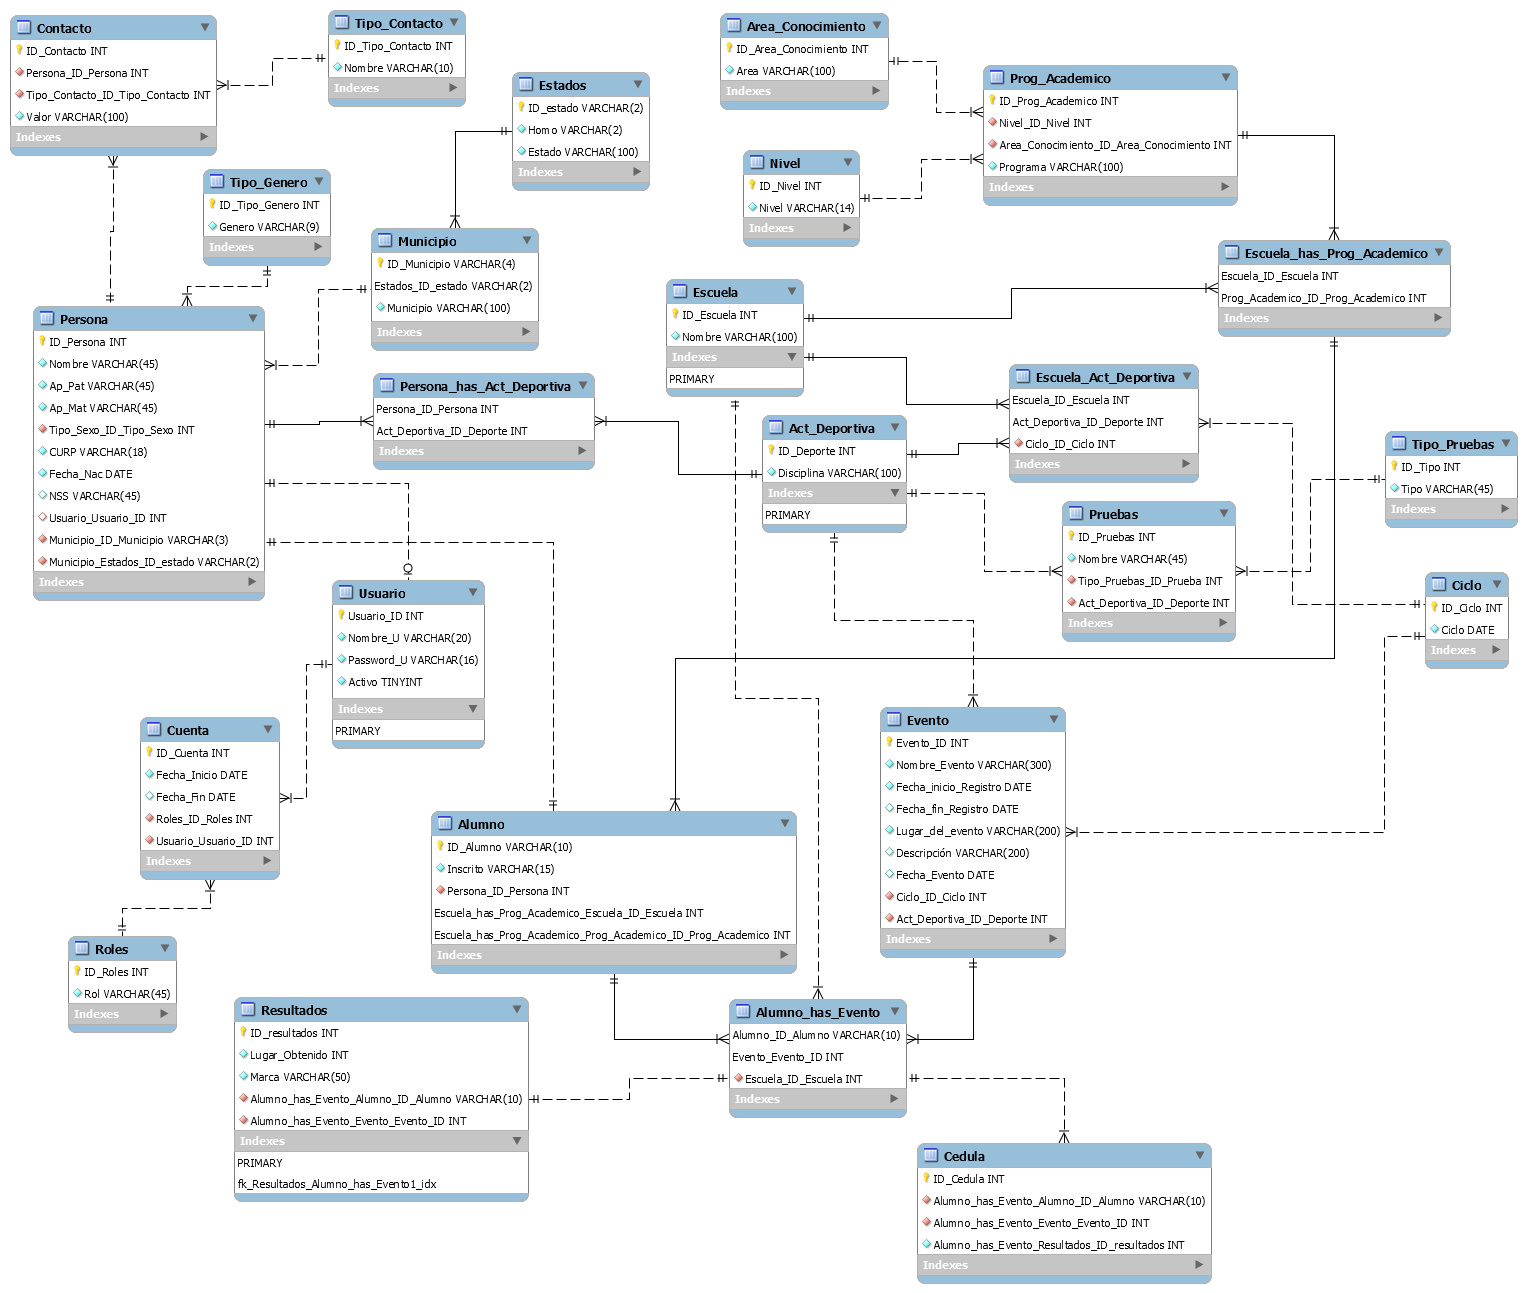
\includegraphics[angle=90, width=10cm, height=15cm]{Imagenes/BasedeDatos}
		\caption{Base de Datos propuesta en Trabajo Terminal 1.}
		\label{basededatosInicial}
	\end{figure}
	
	\noindent Los cambios realizados fueron respecto a la tabla de Tipo de Contacto, esta se cambio por la separación del tipo de contacto. Quedando tres tablas nuevas, las cuales son: Telefonono Fijo, Telefonono Celular y extensión. \\
	Otro cambio realizado fue la relación entre la tabla Evento y la tabla Act Deportiva, con el cambio realizado quedó la tabla Evento relacionada con la tabla Prueba. Con la finalidad de encontrar especifícamente los datos de un evento en particular, ya que nos percatamos que con la primer relación se mostraban datos duplicados. 
	
	%=========================================================
	%                                                         Sprint 1
	%=========================================================
	\section{Sprint 1:  Mecanismo de validación de estatus académico.}
	\noindent Para el desarrollo de este Sprint se desarrolla la forma de verificar el estatus académico de los alumnos que deseen participar en un evento interpolitécnico. \\
	Dicha verificación consiste de 3 pasos:
	\begin{enumerate}
		\item Ingresa credenciales en la aplicación web RIDESCOM.
		\item Se verifican credenciales en el SAES.
		\item Accede a la página RIDESCOM.
	\end{enumerate}
	
	Como primer paso, el usuario ingresa el usuario y contraseña, mismas que ocupa para ingresar al Sistema de Administración Escolar SAES.
	Una vez ingresado Usuario y Contraseña, la aplicación hace uso del Crawler \ref{crawler}. \\
	Este tomará la información de Usuario y Contraseña, las utilizará para ingresar al SAES, de tal manera que se comprobará si estas son correctas o no. En cualquier caso, se tomará la respuesta para mostrala al usuario.
	Finalmente, en la aplicación web se buscará la respuesta del Crawler para definir el acceso a la aplicación.
	
	El objetivo de este mécanismo es comprobar la inscripción del alumno en el IPN, ya que en el reglamento en el que se basan los eventos interpolitécnicos deportivos, donde se menciona que solo deben participar alumnos que estén inscritos. \ref{crawler}
	
	
	%=========================================================
	%                                                         Sprint 2
	%=========================================================
	\section{Sprint 2: Interfaces}
	\noindent Para la desarrollo de este SPRINT se tomaron los debidos requerimientos para la realización del diseño de las interfaces y así hacer que la aplicación sea amigable con el usuario utilizando las siguientes plantillas para la visualización de las interfaces como una propuesta.
	\newline
	
	\noindent Interfaz Inicio general: Esta interfaz es la principal donde los usuarios podrán visualizar datos de aspecto público. 
	\newline
	Parte 1:
	Cualquier usuario que visite la URL de la aplicación podrá ver los elementos de navegación tales como: Inicio (Página principal), Registro, Calendario, Inicia Sesión, Contacto, los deportes que se imparten en la ESCOM, una introducción a los eventos interpolitécnicos deportivos próximos, como se muestra en la Figura \ref{inicioGeneral}. 
	\newline
	\begin{figure}[hbt!]
		\centering
		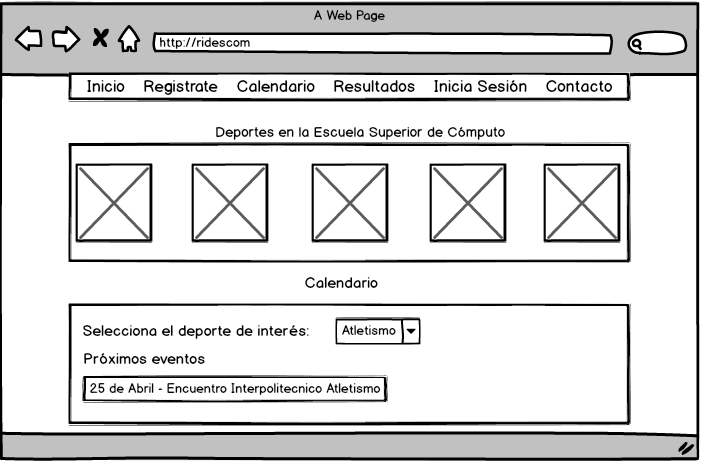
\includegraphics[width=10cm, height=6cm]{Imagenes/Disenos/Iniciogeneral}
		\caption{Inicio general}
		\label{inicioGeneral}
	\end{figure}
	
	Parte 2:
	Dentro de la misma habrá una sección de resultados generales de los últimos eventos realizados y finalmente una  sección donde se localiza el contacto del plantel para más información al respecto y un contacto de Facebook del área de actividades deportivas de la ESCOM, para mas detalles consulte en el apartado Anexo la Figura \ref{inicioGeneral1}.
	\pagebreak
	
	\begin{figure}[hbt!]
		\centering
		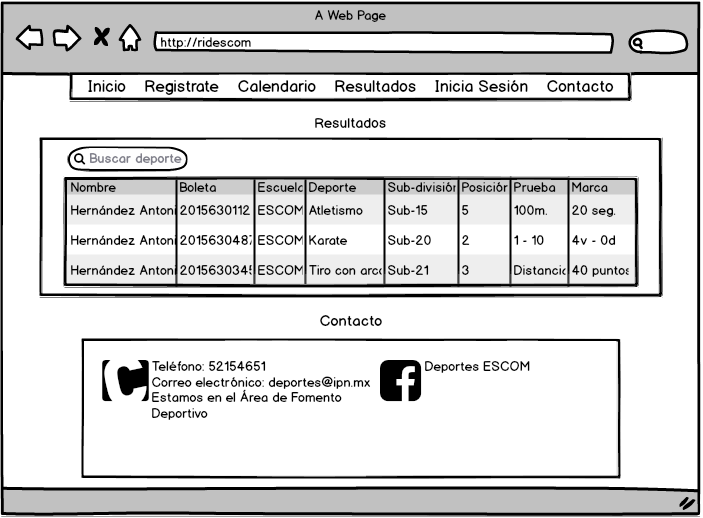
\includegraphics[width=10cm, height=6cm]{Imagenes/Disenos/Iniciogeneral1}
		\caption{Inicio General parte 2}
		\label{inicioGeneral1}
	\end{figure}
	
	\noindent Interfaz Login del Jefe del Departamento de Fomento Deportivo: En esta interfaz ayuda al usuario indicando los elementos que se necesitan para iniciar sesión como usuario de la aplicación (Nombre-Usuario/contraseña previamente registrado), si el usuario no existe el mecanismo realizado en el SPRINT1 se encargará de rechazarlo, podrá recuperar su contraseña en la sección de “¿Olvidaste tu contraseña?”, para mas detalles consulte en el apartado Anexo la Figura 	\ref{inicioJFDycoord}. 
	\newline
	
	\noindent Interfaz Inicio del Jefe del Departamento de Fomento Deportivo: El diseño de la página será muy similar con el resto de los usuarios, sin embargo, este contará con distintas opciones como son: Crear un evento deportivo, Resultados, Calendario y Control de cordinadores donde en este apartado tendrá la opción de Consultar coordinadores, Registrar usuario, Modificar contraseña de los coordinadores de las Unidades Académicas, para mas detalles consulte en el apartado Anexo la Figura 	\ref{principalJFD}. El diseño en general de la vista de este usuario se puede ver en el apartado Anexo \ref{diseños} las Figuras \ref{principalJFD} y \ref{principalJFD1}.
	\newline
	
	\noindent Interfaz Crear un evento interpolitécnico: Dentro de esta vista el Jefe del Departamento de Fomento Deportivo llenaráa los campos para poder dar de alta algún evento, se pedirá el Nombre del evento, Fecha en la que se llevará acabo, Fecha inicio de inscripción y Fecha fin de inscripción, un campo de Descripción donde podrá agregar la dirección del lugar entre otros datos. Se seleccionará el deporte al que corresponde dicho evento, para mas detalles consulte en el apartado Anexo \ref{diseños} la Figura \ref{creaevento}.
	\newline
	
	\noindent Interfaz Registra un coordinador: Se solicitarán datos como Nombre, Apellido Paterno, Apellido Materno,correo electrónico, teleéfonos de contacto y Escuela a la que pertenece, para mas detalles consulte en el apartado Anexo \ref{diseños} la Figura \ref{registrarcoord}.
	
	\noindent Interfaz login coordinador: En esta interfaz ayuda al usuario indicando los elementos que se necesitan para iniciar sesión como usuario de la aplicación (Nombre-Usuario/contraseña previamente registrado), si el usuario no existe el mecanismo realizado en el SPRINT1 se encargará de rechazarlo, para mas detalles consulte en el apartado Anexo \ref{diseños} la Figura \ref{inicioJFDycoord}. En caso de que el coordinador olvide su contraseña deberá ponerse en contacto con el Jefe del Departamento de Fomento Deportivo para solicitar el cambio de contraseña.
	\newline
	
	\noindent Interfaz  Inicio del coordinador de una Unidad Académica: Al igual que el resto de los usuarios en general tiene un diseño muy similar, la diferencia recae en las opciones que puede realizar, en este caso son: Registrar entrenador, Calendario, Resultados, Consulta de inscripciones y Válidar perfil, para mas detalles consulte en el apartado Anexo \ref{diseños} la Figuras 	\ref{principalcoord} y en la Figura \ref{principalcoord1} se puede observar que estará disponible un apartado para publicar algun evento previamente dado de alta en la red social de Facebook.
	\newline
	
	\noindent Interfaz Resultados: Este módulo esta designado para que se ingresen los resultados de los participantes y sean vistos en la página principal. Podrá ingresar hasta 20 datos por vez, para mas detalles consulte en el apartado Anexo \ref{diseños} la Figura \ref{ingresaresultados}.
	\newline
	
	\noindent Interfaz Registro entrenador: En este  módulo el coordinador deberá los campos solicitados tales como: No. Empleado, Nombre, Apellidos, Correo electrónico, Teléfono fijo, Teléfono móvil, asi como definir a que deporte pertenece y por ultimo, especificar si cuenta con un asistente, para mas detalles consulte en el apartado Anexo \ref{diseños} la Figura \ref{registroentrenador}.
	\newline
	
	\noindent Interfaz Login alumno: En esta interfaz ayuda al usuario indicando los elementos que se necesitan para iniciar sesión como usuario de la aplicación (Usuario/contraseña previamente registrado), si el usuario no existe el mecanismo realizado en el SPRINT1 se encargará de rechazarlo, podrá recuperar su contraseña en la sección de “¿Olvidaste tu contraseña?”, para mas detalles consulte en el apartado Anexo \ref{diseños} la Figura \ref{loginalumno}.
	\newline
	
	\noindent Interfaz Inicio del alumno: El diseño de la página será muy similar con el resto de los usuarios, sin embargo, este contará con distintas opciones como son: Inscribir un Interpolitécnico, Calendario, Consulta tus registros y Contacto, como se muestra en el apartado Anexo \ref{diseños}, la Figura 	\ref{principalalum}. El diseño en general de la vista de este usuario, para mas detalles consulte en el apartado Anexo \ref{diseños} la Figuras \ref{principalalum} y \ref{principalalum1}.
	\newline
	
	\noindent Interfaz Inscribir interpolitécnico: En este módulo el alumno primero deberá válidar el estatus de su inscripción, si esta inscrito en el periodo actual, se habilitará el botón para registrar la cédula. En caso contrario el botón no estará habilitado y por tanto, no podrá inscribirse. Los campos que debera llenar el alumno serán: Grupo, NSS (Número de Seguro Social), Lugar de Nacimiento, correo electrónico, Delegación/Municipio, asi como seleccionar el deporte, sub-division y prueba en la que quiere participar, para mas detalles consulte en el apartado Anexo \ref{diseños} las Figuras \ref{Inscripcioninterpolitecnico}.
	\newline
	
	\noindent Interfaz Consulta tus registros: En este módulo, el participante podrá visualizar en una tabla los eventos a los cuales se a registrado, a su vez le mostrará información como: el deporte, prueba Fecha del Evento y la direccion del mismo, para mas detalles consulte en el apartado Anexo \ref{diseños} la Figura \ref{consultainscripcion}.
	\newline
	
	\noindent En este capítulo se presentará una breve descripción del trabajo realizado, los problemas que se enfretaron, así como lo que se logró. Continuando con el capítulo se presentan los Sprint porgramado. 
	De manera breve se hace mención de los casos de uso desarrollados, vistas del proyecto final. así como las pruebas realizadas.
	
	\section{Sprint 3: Módulo de formulario}	
	\noindent En el desarrollo de este Sprint se desarrollaron los formulario necesario para el proyecto, sin embargo, en el proceso de desarrollo se optó por implementar un Crawler, el cual ayudaría a reducir vistas y manejo de información al comprobar los datos de un alumno. Siendo así, los formularios desarrollados son: agregar, editar y eliminar deporte, agregar, editar y eliminar coordinador de unidad académica, agregar, editar y eliminar evento, agregar, editar y eliminar pruebas, inscribir interpolitecnico.
	
	\section{Sprint 4: Módulo de difusión de eventos}
	\noindent Este Sprint se planteó mostrar a los usuarios involucrados en la aplicación web los eventos disponibles al momento, siendo así puedan informarse y decidir los eventos en los que quiera participar. Durante el proceso de desarrollo en Trabajo Terminal 2, se modificó la manera en la que se presentaría estos. 
	En un principio se planteó en mostrar los datos dentro de una tabla como se muestra en la Figura  , sin embargo esto cambió de tal manera que se presentará los datos de cada evento en un recuadro y a su vez estos están ordenados de forma ordenada.
	\pagebreak
	
	\section{Sprint 5:Módulo de comunicación con redes sociales}	
	\noindent Este Sprint se planteó con la finalidad de hacer llegar por distintos medios, los eventos que están disponibles para su inscripción. De tal manera, se estableció que estos fueran compartidos a través de la red social Facebook.
	Teniendo en cuenta lo antes mencionado, se utiliza la API de Facebook la cual proporciona tanto la documentación, ejemplos y herramientas para que puedan ser ocupadas para su integración en distintos proyectos. \\
	\noindent Lo que se desarrolló fue el iniciar sesión desde la aplicación web “Ridescom”, una vez ingresada a la cuenta se puede realizar la publicación de los distintos eventos desde la misma, viendo reflejado el cambio directamente en el apartado de publicaciones de la página correspondiente en Facebook. \\
	\noindent Para lograr esto como primer paso se creó una cuenta de correo electrónico. Se estableció un correo y contraseña, esto servirá para posteriormente crear una cuenta en la red social de Facebook y a su vez, hacer uso de las herramientas de desarrollo de Facebook.
	A continuación se muestra el momento y datos que se pusieron para crear el correo electrónico.
	
	\begin{figure}[hbt!]
		\centering
		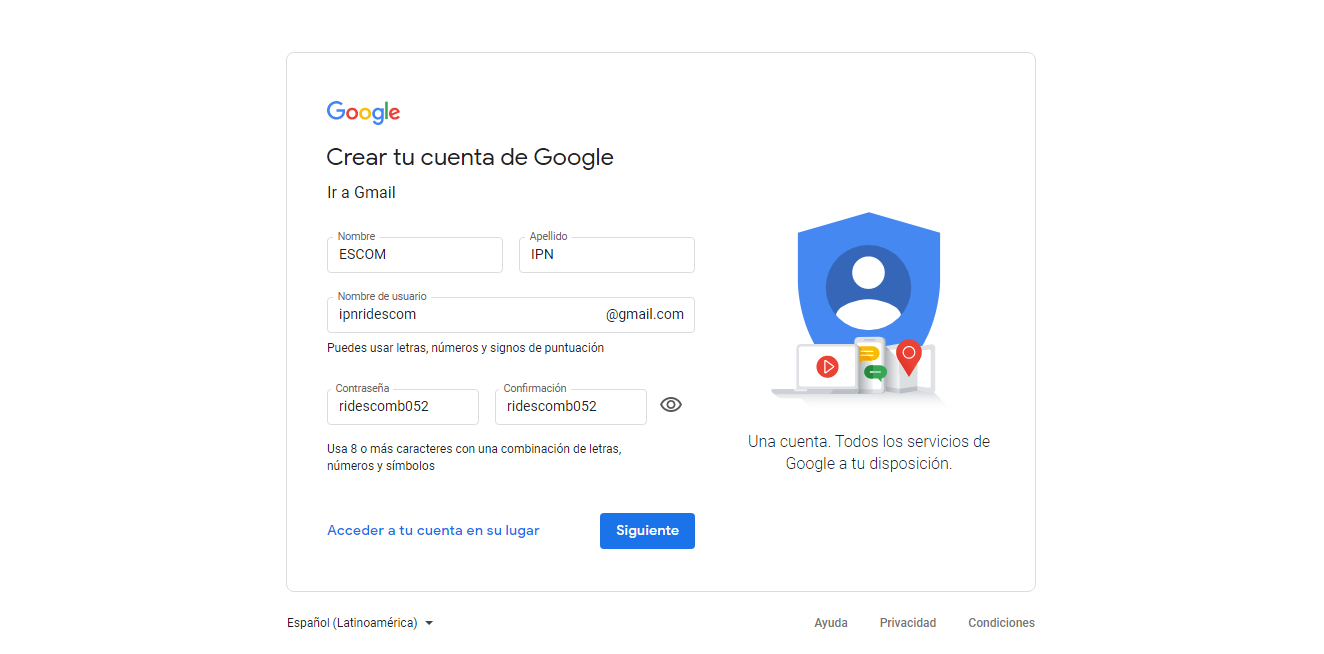
\includegraphics[width=12cm, height=6cm]{Imagenes/CreacionCuentaFB/CuentaGmail}
		\caption{Creacion de la cuenta en Gmail.}
		\label{cuentagmail}
	\end{figure}
	
	
	\noindent Posteriormente se creó la cuenta en la red social facebook, ya que es necesario crear una página en la antes mencionada para la difusión de los eventos. 
	
	\begin{figure}[hbt!]
		\centering
		
\includegraphics[width=10cm, height=6cm]{Imagenes/CreacionCuentaFB/CreacionCuentaFB}
		\caption{Creación de cuenta en la red social Facebook.}
		\label{creacioncuentafb}
	\end{figure}
	\pagebreak
	
	\noindent Una vez teniendo la cuenta creada se creó la página que se utilizará para la difusión de los eventos. Como se muestra a continuación.
	
	\begin{figure}[hbt!]
		\centering
		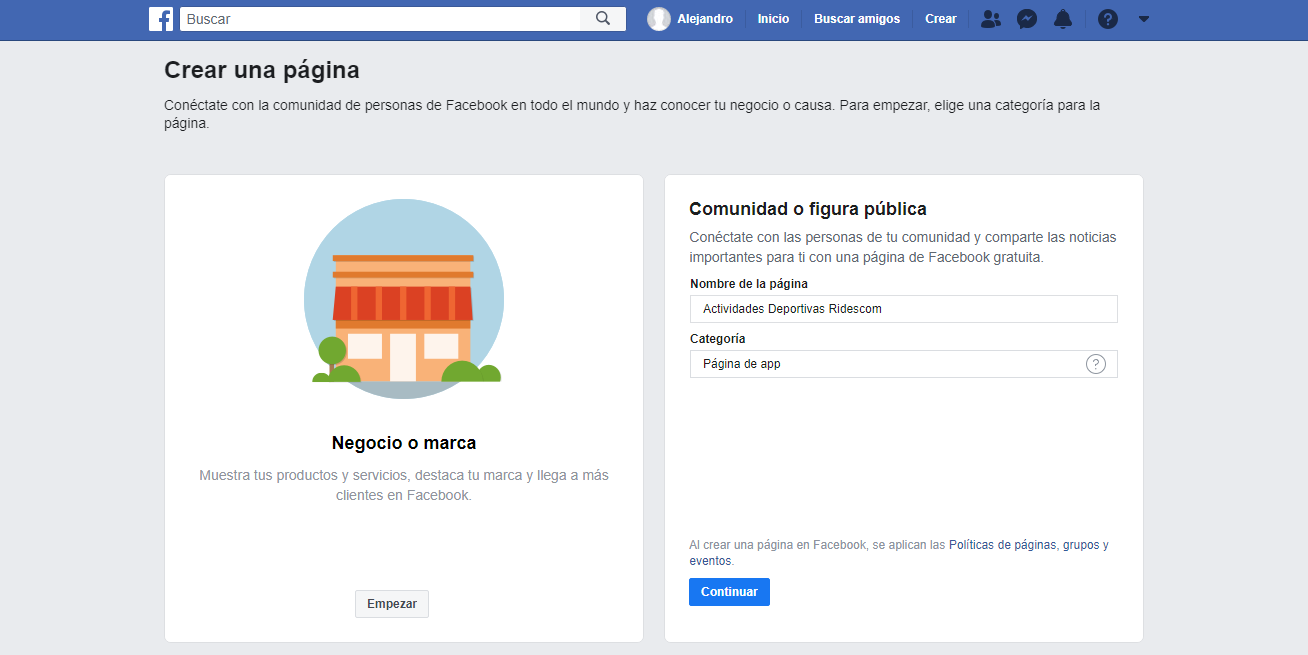
\includegraphics[width=10cm, height=6cm]{Imagenes/CreacionCuentaFB/CreacionPagina}
		\caption{Creación página en Facebook.}
		\label{creacionpagina}
	\end{figure}
	
	
	\noindent Teniendo creada la cuenta y la página en Facebook, desde le herramienta Developers Facebook, se crea una aplicación, la cual tendrá como función el enviar los datos entre nuestra aplicación y la página de Facebook.\\
	
	\noindent Para realizar dicha conexón se accede a la configuración de la aplicación, para que la página que se creó previamente aparezca como una opción para conectar, debe de incluir el nombre de la aplicación (creada en Developers) y en el apartado de categoría se debio seleccionar la opcion de Página de app como se muestra en la Figura \ref{creacionpagina}.
	
	\noindent Al concluir con el proceso de ligar la página de Facebook con la aplicación se muestra el cambio, como se puede apreciar en la Figura \ref{conexionpaginaapp}.
	
	\begin{figure}[hbt!]
		\centering
		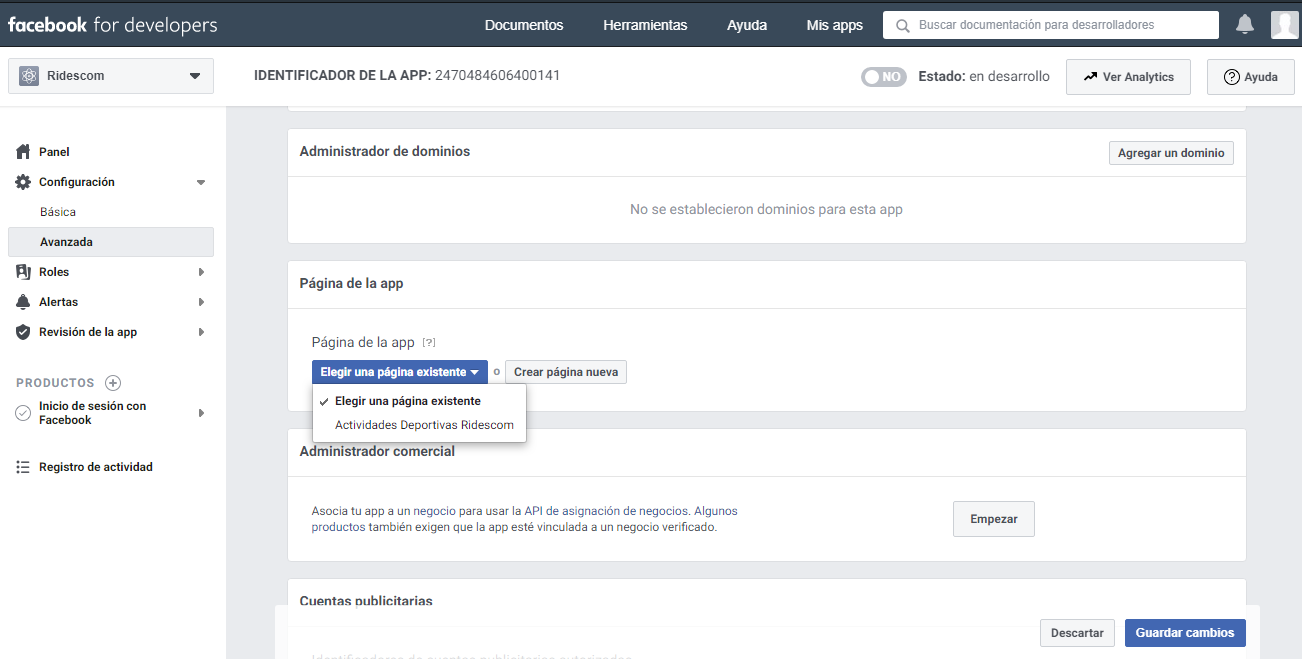
\includegraphics[width=10cm, height=6cm]{Imagenes/CreacionCuentaFB/ConexionPagina}
		\caption{Conexión entre página y aplicación.}
		\label{conexionpaginaapp}
	\end{figure}
	
	
	\noindent Sin embargo, durante el periodo correspondiente a Trabajo Terminal 2 los términos de uso se actualizaron solicitando datos por verificar para poder hacer uso de las herramientas de Facebook. A su vez se cambió la estructura y envío de  datos para una correcta conexión entre las herramientas de Facebook y el proyecto que se está desarrollando, para más detalles consulte el apartado \ref{apiFB}.
	\pagebreak
	
	\section{Sprint 6:Módulo de creación de cédula de inscripción.}
	\noindent Este Sprint se planteó ya que un problema es que se inscribían personas fuera del IPN, con esto se genera automaticamente un listado donde vienen los alumnos inscritos en cada uno de los eventos.
	Para el desarrollo de este módulo se realizó una investigación de un pluggin o herramienta que sea compatible y de fácil implementación para la generación de un reporte. Una vez realizada la investigación se decidió usar la herramienta iReport, la cual tiene facilidad al integrarla al proyecto y facilidad al hacer uso de la misma. Una vez agregado el pluggin que nos permite hacer uso de la misma, se hizo de un análisis de los parámetros que se iban a mostrar en el reporte. Se definió un formato único que será utilizado por las distintas Unidades Académicas, a su vez se definió que será en formato PDF ya que así, se puede apoyar a la mitigación de edición de datos de los participantes. Al descargar el formato, el Coordinador podrá visualizar un listado de los participantes que se inscribieron en algún evento iterpolitécnico deportivo durante las fechas establecidas.
	
	
	\section{Sprint 7: Módulo de consulta de resultados.}
	\noindent Este Sprint se planteó con la finalidad de que los actores involucrados en la aplicación web puedan visualizar los resultados obtenidos por los alumnos participantes en los eventos interpolitécnicos deportivos. 
	Estos se mostrarán en una tabla con los datos más relevantes de estos, cabe destacar que se agrega un módulo para el participante el cual es “Historial”, la finalidad de este es para que el alumno pueda ver de manera fácil y rápida los eventos en los que a participado a lo largo de su trayectoria académica complementando con los datos relacionados a los resultados de los mismos.